%% 
%% Copyright 2007, 2008, 2009 Elsevier Ltd
%% 
%% This file is part of the 'Elsarticle Bundle'.
%% ---------------------------------------------
%% 
%% It may be distributed under the conditions of the LaTeX Project Public
%% License, either version 1.2 of this license or (at your option) any
%% later version.  The latest version of this license is in
%%    http://www.latex-project.org/lppl.txt
%% and version 1.2 or later is part of all distributions of LaTeX
%% version 1999/12/01 or later.
%% 
%% The list of all files belonging to the 'Elsarticle Bundle' is
%% given in the file `manifest.txt'.
%% 
%% Template article for Elsevier's document class `elsarticle'
%% with harvard style bibliographic references
%% SP 2008/03/01

\documentclass[preprint,12pt,authoryear]{elsarticle}

%% Use the option review to obtain double line spacing
%% \documentclass[authoryear,preprint,review,12pt]{elsarticle}

%% Use the options 1p,twocolumn; 3p; 3p,twocolumn; 5p; or 5p,twocolumn
%% for a journal layout:
%% \documentclass[final,1p,times,authoryear]{elsarticle}
%% \documentclass[final,1p,times,twocolumn,authoryear]{elsarticle}
%% \documentclass[final,3p,times,authoryear]{elsarticle}
%% \documentclass[final,3p,times,twocolumn,authoryear]{elsarticle}
%% \documentclass[final,5p,times,authoryear]{elsarticle}
%% \documentclass[final,5p,times,twocolumn,authoryear]{elsarticle}

\usepackage{hyperref}
\hypersetup{
  colorlinks   = true, %Colours links instead of ugly boxes
  urlcolor     = blue, %Colour for external hyperlinks
  linkcolor    = blue, %Colour of internal links
  citecolor   = red %Colour of citations
}

%% For including figures, graphicx.sty has been loaded in
%% elsarticle.cls. If you prefer to use the old commands
%% please give \usepackage{epsfig}
\usepackage{subfig}

%% The amssymb package provides various useful mathematical symbols
\usepackage{amssymb}
%% The amsthm package provides extended theorem environments
%% \usepackage{amsthm}

%% The lineno packages adds line numbers. Start line numbering with
%% \begin{linenumbers}, end it with \end{linenumbers}. Or switch it on
%% for the whole article with \linenumbers.
%% \usepackage{lineno}

\journal{Applied Mathematics and Computation}

%commands:
\newcommand{\fig}[1]{\hyperref[#1]{Fig.\ref{#1}}}

%math:
\newcommand{\dd}{\; \mathrm{d}}

\begin{document}

\begin{frontmatter}

%% Title, authors and addresses

%% use the tnoteref command within \title for footnotes;
%% use the tnotetext command for theassociated footnote;
%% use the fnref command within \author or \address for footnotes;
%% use the fntext command for theassociated footnote;
%% use the corref command within \author for corresponding author footnotes;
%% use the cortext command for theassociated footnote;
%% use the ead command for the email address,
%% and the form \ead[url] for the home page:
%% \title{Title\tnoteref{label1}}
%% \tnotetext[label1]{}
%% \author{Name\corref{cor1}\fnref{label2}}
%% \ead{email address}
%% \ead[url]{home page}
%% \fntext[label2]{}
%% \cortext[cor1]{}
%% \address{Address\fnref{label3}}
%% \fntext[label3]{}

\title{Partition of unity methods for approximation of point water sources in~porous media}

%% use optional labels to link authors explicitly to addresses:
%% \author[label1,label2]{}
%% \address[label1]{}
%% \address[label2]{}

\author{Pavel Exner}
\ead{pavel.exner@tul.cz}
\ead[url]{https://github.com/Paulie14/xfem\_project}
\address{Technical University of Liberec, Studentsk{\' a} 1402/2, 461 17 Liberec 1, Czech Republic}

\begin{abstract}
%% Text of abstract
In this work we demonstrate usage of Partition of Unity (PU) methods to improve approximation of singularities 
in the solution of the Poisson equation. The model that we solve describes a steady flow of water in an aquifer
which consists of porous media. The aquifer is perforated by wells and boreholes which are often represented
as point sources considering their small diameter and the vast size of the aquifer. This brings singularities 
into the solution. The extended and stable generalized finite element method (XFEM and SGFEM) were implemented 
to solve the problem and a proper adaptive integration strategy was developed to gain optimal convergence rates.
\end{abstract}

\begin{keyword}
%% keywords here, in the form: keyword \sep keyword
PUM \sep XFEM \sep SGFEM \sep adaptive integration \sep point sources

%% PACS codes here, in the form: \PACS code \sep code

%% MSC codes here, in the form: \MSC code \sep code
%% or \MSC[2008] code \sep code (2000 is the default)

\end{keyword}

\end{frontmatter}

%% \linenumbers

%% main text
\section{Introduction}
\label{sec:introduction}

People often consider in their models of flow in porous media very large areas which can contain various 
phenomena of very small scale compared with the size of the areas. These can be some disruptions of the porous 
media, e.g. cracks and wells, or material inhomogeneities that cause large gradients in pressure head and 
velocity or even their discontinuities.

Using the standard finite element method (FEM) we are unable to properly approximate the quantities in the 
vicinity of these disturbances, unless we introduce elements of the same scale in the mesh. This leads to 
higher requirements on mesh processing (refinement) and increase of computational costs due to growing number  
of degrees of freedom.

In this work we use PU (Partition of Unity) methods to overcome these problems and demonstrate it on a steady 
%quasi-three-dimensional model of multi-aquifer system 
two-dimensinal aquifer model containing hydro-geological wells which cause singularities in solution. 
We follow the work of~\cite{gracie} who have already used the XFEM (eXtended FEM) on a~similar model. 
However, we focus mainly on the study and improvement of the PU methods, in particular the XFEM (and its 
corrected version) and the SGFEM. 
 
All the implementation was done in C++ language using the Deal II library~\citep{deal}, the finite element library.

\section{Model}
\label{sec:model}
We consider steady flow in a system of aquifers (2D layers of given thickness) which are separated by layers with low permeability (aquitards). 
We suppose the aquitards to be impermeable and so we do about the outer boundary of the aquifers to prescribe homogeneous Neumann 
boundary condition there. 

The distribution of pressure head in $m$-th aquifer is described by Poisson equation
\begin{equation} 
-T^m\Delta{}h^m = f^m  \qquad \textrm{on } \Theta^m,\; \forall m=1,\dots,M, \label{eqn:poisson}
\end{equation}
where $T^m\, [\textrm{m}^2\textrm{s}^{-1}]$ denotes transmisivity, $h^m\, [\textrm{m}]$ pressure head 
and $f^m\, [\textrm{m}\textrm{s}^{-1}]$ source density. Equation (\ref{eqn:poisson}) is derived from the Darcy law and
the continuity equation for incompressible fluid.

The communication between aquifers is possible only through wells which can be seen as 1D problems governed by following equation
\begin{eqnarray} 
\int_{\partial{}B_w^m}\sigma_w^m \left(h^m - H_w^m\right) \, \mathrm{d}\mathbf{x} = c_w^{m+1}\left( H^m_w-H_w^{m+1}\right) - c^m_w\left( H^{m-1}_w-H^m_w \right),
\label{eqn:well_eqs_test} \\
 \forall m=1,\dots,M \;\textrm{ and } \forall w=1,\dots,W, \nonumber
\end{eqnarray}
where $\sigma^m_w\, [\textrm{m}\textrm{s}^{-1}]$ denotes the permeability coefficient between $w$-th well and $m$-th aquifer, 
$H_w^m$ pressure head in the well $w$ at the level of $m$-th aquifer, $c^m_w\, [\textrm{m}^2\textrm{s}^{-1}]$ 
permeability of the well $w$ between aquifers and finally $\partial{}B^m_w$ is the boundary of the well.
The equation (\ref{eqn:well_eqs_test}) puts the flow in and out of the well on right hand side and the flow through
the well boundary on the left hand side in balance.

The transfer between wells and aquifers can be treated in two ways. There is a well boundary integral on the left hand side of (\ref{eqn:well_eqs_test}) 
and it represents flow over the boundary of the well. Second variant uses a surface integral in (\ref{eqn:well_eqs_test}) which represents flow source
in the area of aquifer and well cross-section (the units of $\sigma^m_w$ then changes). The same integral appears also in the weak formulation 
of (\ref{eqn:poisson}) -- as a boundary integral in the first variant or as a part of the source term in the second variant.
Both variants were tested in the work with nearly identical results, only the second approach simplifies the implementation and slightly speeds up the assembly.



\section{PUM methods}
\label{sec:pum_methods}

\section{Integration on enriched elements}
\label{sec:integration}

The higher requirements on integration precision
%TODO: integration of term in what equation
are the price for using enrichment functions and a coarse mesh.
We need to deal with integration of enrichment functions which can be non-polynomial, as they are in our case. 
The standard quadrature rules are not appropriate any more, as they are constructed to integrate precisely 
polynomials up to a given degree. 

There are two aspects which the adaptive integration must handle properly and integrate precisely enough:
\begin{itemize}
  \item the singularity and the steep gradient of the pressure head in the vicinity of a well,
  \item the weak discontinuity of the pressure head at the well edge (jump in the pressure head gradient).
\end{itemize}

%TODO: better quadrature for log is not proper in our case as the function may be different according to hydrogeologist
One of the approaches to improve integration is local element refinement. We remind that the refinement helps
only placing more quadrature points in the element and does not bring any more degrees of freedom in the 
system. We will discuss the criterions for adaptive refinement, suggest improvement and compare our solution
with the original one in this subsection. We will refer also some of the convergence results which will be 
shown later in \ref{sec:results}.

\subsection{Adaptive refinement of an element}
\label{sec:refinement_element}

\cite{gracie} used a criterion for adaptive refinement according to which only the subelements 
that have nonzero cross-section with the well are refined. This catches nicely the well edge but it can work 
well only in some special cases when the well is at the node of an element or near the center of an element. 
The problem comes when the well is placed near the edge or node of an element. In that case there can be
large difference in the size of neighbouring subelements as you can see in \fig{fig:adapt_ref_a}. Although
the integrand is computed precisely enough on the element with the well inside, the quadrature points on the
neighbouring elements (where the pressure head gradient can be still large) are placed very sparsely 
and the integration error is large.

\begin{figure}[!htb]
%   \vspace{0pt}
  \centering    
  \subfloat[original refinement]{\label{fig:adapt_ref_a} 
    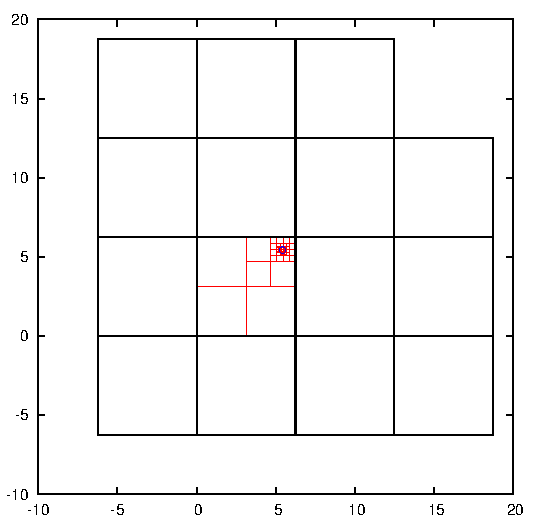
\includegraphics[width=0.45\textwidth]{results/adaptive_refinement_3_old.pdf} }
  \hspace{0pt}
  \subfloat[improved refinement]{\label{fig:adapt_ref_b} 
    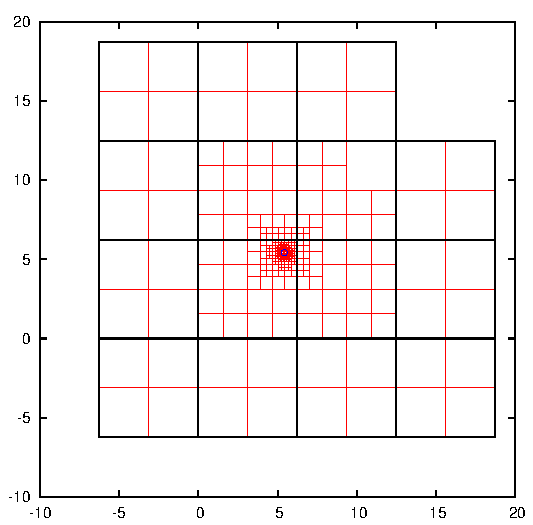
\includegraphics[width=0.45\textwidth]{results/adaptive_refinement_3_new.pdf} }
  \caption[Adaptive refinement comparision]
  {Comparision of different refinement techniques.
   Black lines denote element edges, red lines denote adaptive refinement (subelement edges) and the well
   edge is blue.
  }
  \label{fig:adapt_refinement}
\end{figure}

We suggested additional criterion for subelements refinement which takes into account a subelement diameter 
and its distance from the well
\begin{equation}
  d_T > C_R|d_{min} - r_w|,
\end{equation}
where $d_T$ is the diameter of the subelement and $d_{min}$ is minimal distance between a vertex of 
the subelement and the well edge. $C_R$ is a scaling constant, equal 1.0 by default, through which we can 
control the significance of the criterion.

In this way, the elements in which the well does not lie are also refined as you can see in 
\fig{fig:adapt_ref_b}. The quadrature points are then distributed more 'smoothly' around the well and the
gradients can be computed more accurately. 

In \fig{fig:adapt_refinement_norm} you can see the $L_2$ norms of the error on the enriched elements which 
were computed also using the corresponding adaptive integration. Notice the scale of the improved version -- 
the error on elements is in small range and is not significantly concentrated anywhere. On the other hand, 
the original version shows out large error that is concentrated on the closest non-refined element to the well.

%TODO: number of quadrature points in both approaches

\begin{figure}[!htb]
%   \vspace{0pt}
%TODO: add axis, remove legend label, try to sharpen
  \centering    
  \subfloat[original refinement]{\label{fig:adapt_ref_norm_a} 
    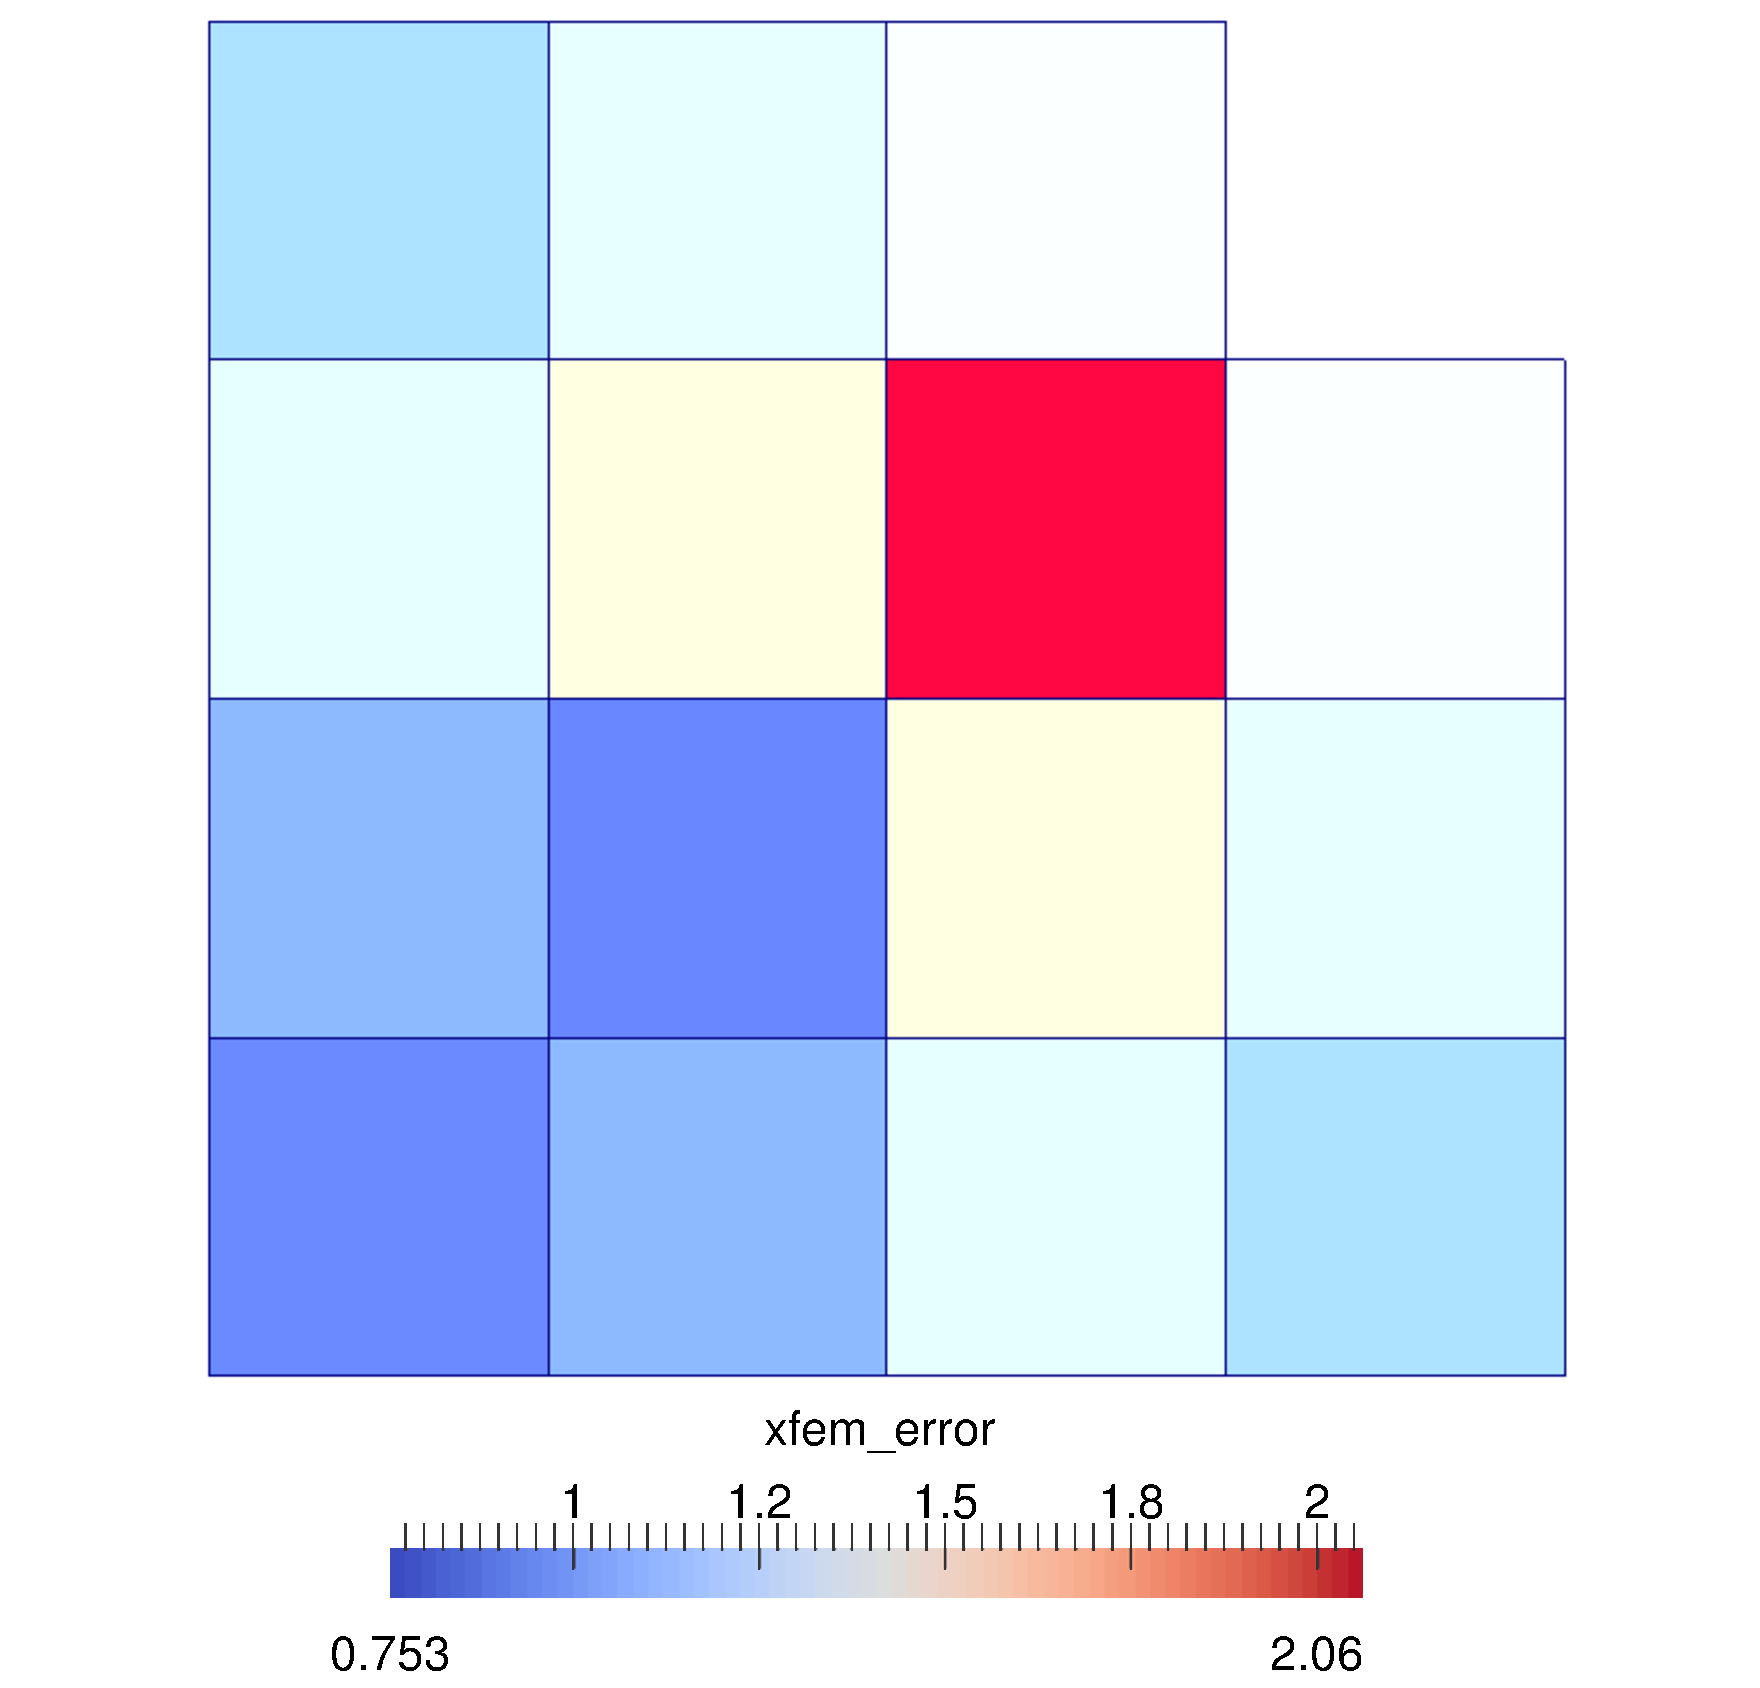
\includegraphics[width=0.45\textwidth]{results/adaptive_refinement_extract_3_old.pdf} }
  \hspace{0pt}
  \subfloat[improved refinement]{\label{fig:adapt_ref_norm_b} 
    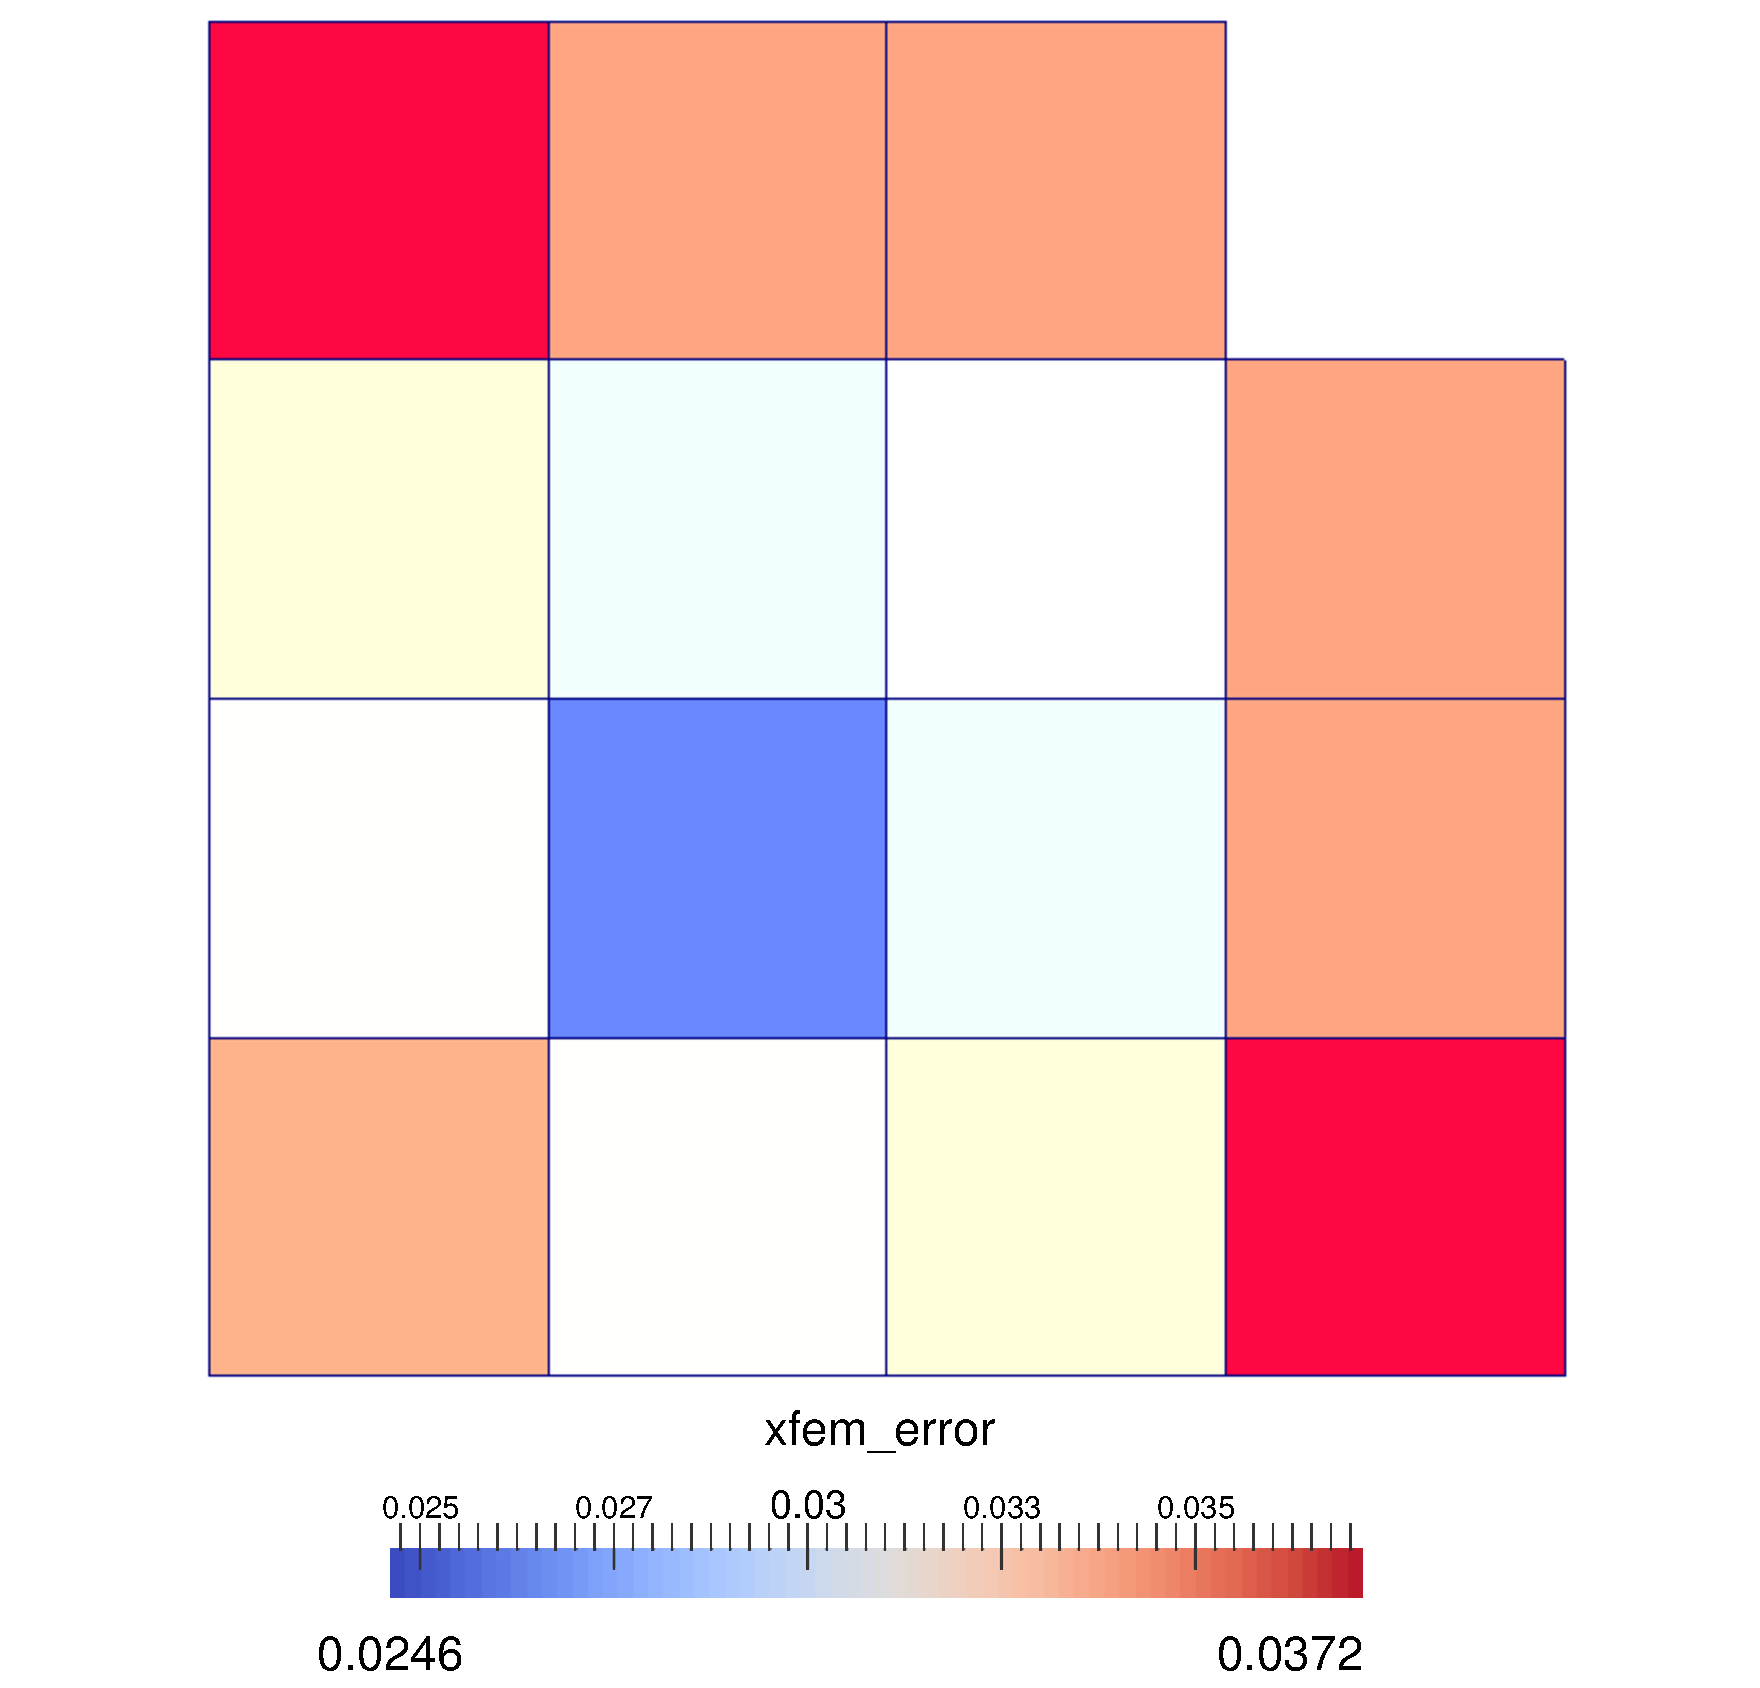
\includegraphics[width=0.45\textwidth]{results/adaptive_refinement_extract_3_new.pdf} }
  \caption[Adaptive refinement comparision]
  {Comparision of elementwise error in $L_2$ norm using different refinement techniques.
  }
  \label{fig:adapt_refinement_norm}
\end{figure}


\subsection{Circle integration experiment}
The approximation of the integration domain is also the source of the error. We decided to run 
an experiment on integrating the characteristic function of the well with our adaptive integration.
The domain $\Omega$ is a square $4\times4$ out of which a circle of radius 1.0 is cut off. The characteristic 
function is considered
\begin{equation}
  \chi(\mathbf{x}) = \left\{
    \begin{array}{l l}
      0 & \quad \textrm{if } \mathbf{x} \textrm{ is inside the circle}\\
      1 & \quad \textrm{otherwise}
  \end{array} \right.
\end{equation}
and the integral 
\begin{equation}
  \int_{\Omega}\chi(\mathbf{x}) \dd\mathbf{x} = 4^2 - \pi
\end{equation}
is equal the area of the square minus the area of the circle.

In this experiment we investigate the influence of the order of the quadrature rule and the level of
the refinement on how precisely the well geometry is captured.

In the graph in \fig{fig:adapt_ref_convergence} we can see that for all the quadratures the convergence rate
is similar, around 1.5. The gain from using higher order quadratures is not worth, especially in case 
of the order 4 the error is not much smaller than the error of the quadrature of the order 3. 

Finally the highest level of refinement is chosen to be 10 and the quadrature order to be 3. The number of
the quadrature points generated by the process desribed above in \ref{sec:refinement_element} is then similar 
both in the original (14793) and improved version (14819).

\begin{figure}[!htb]
%   \vspace{0pt}
%TODO: add refinement level to legend
  \centering    
  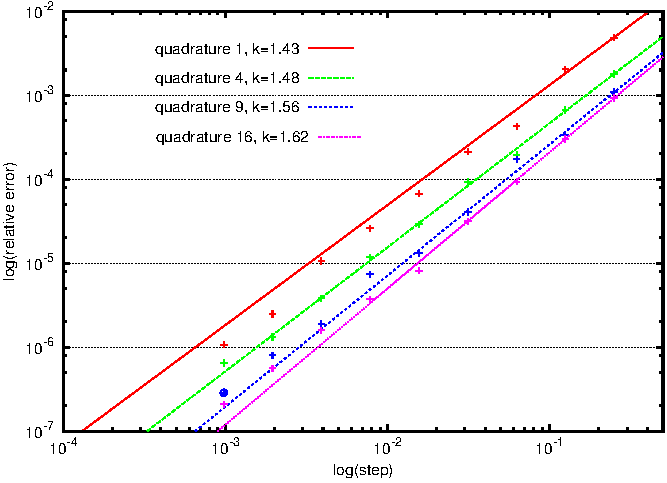
\includegraphics[width=0.7\textwidth]{results/adaptive_integration.pdf}
%   \subfloat[rozdìlený element s vrtem]{\label{fig:adapt_ref_a} 
%     \includegraphics[width=70mm]{\figpath adaptive_ref.pdf} }
%   \hspace{0pt}
%   \subfloat[detail hranice vrtu]{\label{fig:adapt_ref_b} 
%     \includegraphics[width=72mm]{\figpath adaptive_ref_detail.pdf} }
  \caption[Adaptive refinement convergence]{Convergence of adaptive refinement of a circle cutoff.}
  \label{fig:adapt_ref_convergence}
\end{figure}


* non-optimal convergence rate with the approach of [gracie] and their integration scheme 3-4

* the above can be improved by using higher order quadrature rules (6-6)

* problem is that we do not represent the well edge and mainly its surrounding well enough

* introduce element refinement criterion: the comparision of element size and its minimal vertex distance 
  from the well

\section{Results}
\label{sec:results}

\section{Summary}
\label{sec:summary}

\section{Acknowledgement}
This work was made under the sincere guidance and support of Mgr. Jan B{\v r}ezina, Ph.D.

This work was supported by the Ministry of Education of the Czech Republic within the SGS project 
no. 21066/115 on the Technical University of Liberec.

%% The Appendices part is started with the command \appendix;
%% appendix sections are then done as normal sections
%% \appendix

%% \section{}
%% \label{}

%% If you have bibdatabase file and want bibtex to generate the
%% bibitems, please use
%%
%%  \bibliographystyle{elsarticle-harv} 
%%  \bibliography{<your bibdatabase>}

%% else use the following coding to input the bibitems directly in the
%% TeX file.

% \begin{thebibliography}{00}
% 
% %% \bibitem[Author(year)]{label}
% %% Text of bibliographic item
% 
% \bibitem[ ()]{}
% 
% \end{thebibliography}
 %\nocite{dip}
 \bibliographystyle{elsarticle-harv} 
 %\bibliographystyle{elsarticle-num-names} 
 %\bibliographystyle{elsarticle-num} 
 \bibliography{../citace.bib}
\end{document}

\endinput
%%
%% End of file `elsarticle-template-harv.tex'.
